\chapter{Сценарии и эксперименты}

Эксперименты проводятся в мультиагентной среде multiagent-particle-envs \cite{multiagent-particle-envs} от компании OpenAI.


\section{Эксперименты}

\subsection{Эксперимент на одном мозге}

В алгоритме MADDPG каждый агент имеет набор сетей \textit{критиков}, чтобы иметь собственный механизм оптимизации политики. Тем не менее, два агента в \textit{Simple Reference} полностью симметричны в том смысле, что они оба имеют одинаковое пространство наблюдения, пространство действий и имеют общую глобальную награду. Тем самым агенты формулируют аналогичные оптимальные политики.

Таким образом, каждому агенту можно было бы не создавать свой собственный мозг из сетей критиков, а вместо этого тренировать один мозг для всех агентов. Кроме того, единый мозг MADDPG позволяет агентам общаться на одном «языке», что означает, что они произносят и понимают ориентиры в одних и тех же кодировках.

Так же мы разработали вариант этого алгоритма, можно сказать, что в том случае мы имеем два мозга: один для агентов из одной команды, второй – для агентов из другой команды. Этот вариант мы применили к сценарию \textit{Simple Tag}. Это возможно благодаря тому, что агенты из одной команды в этом сценарии имеют одинаковое пространство наблюдения, пространство действий и имеют общую глобальную награду, но это не так для агентов из разных команд. Поэтому и пришлось использовать отдельный набор сетей для каждой команды.

\subsection{Эксперимент с декомпозированным вознаграждением}

Чтобы обеспечить чёткие сигналы для двух независимых поддействий, мы попробовали реализовать отдельные наборы \textit{актор-критиков} для физического движения и общения.

\begin{figure}[ht!]
    \center
    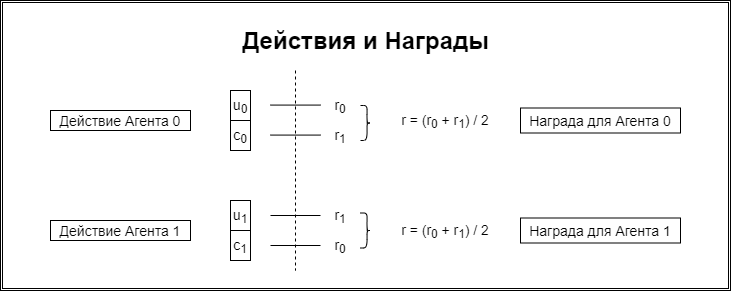
\includegraphics [scale=0.60] {my_folder/images/ch4/actions_and_rewards.png}
    \caption{С левой стороны от пунктирной линии - действие агента, которое представляет собой совокупность физического движения \textit{u} и коммуникационного действия \textit{c}. С правой стороны показано, как награда рассчитывается и назначается для оценки действий. Два агента имеют одинаковую глобальную награду - среднее значение между $r_0$ и $r_1$.}
    \label{fig:action-reward}
\end{figure}

Из \firef{fig:action-reward} видно, что физическое перемещение $u_0$ агента 0 оценивается $r_0$, а высказывание $c_0$ - $r_1$. Окончательное вознаграждение затем раскладывается как кортеж из $r_0$ и $r_1$, т.е. $[r_0; r_1]$, причем каждый элемент соответствует сигналу оценки физического движения и связи соответственно. Точно так же последний набор вознаграждений для агента 1 равен $[r_1; r_0]$.

\begin{figure}[ht!]
    \center
    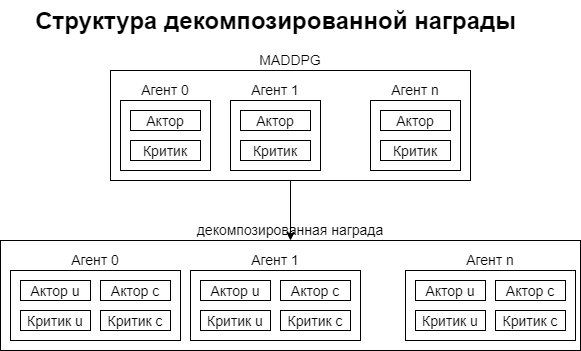
\includegraphics [scale=0.60] {my_folder/images/ch4/decomposed_reward_structure.png}
    \caption{Сетевая структура декомпозированного вознаграждения по сравнению со стандартным MADDPG.}
    \label{fig:decomposed-reward-structure}
\end{figure}

Для физического движения и общения созданы два отдельных набора сетей \textit{актор-критик}, чтобы обеспечить согласованные и точные градиенты для оптимизации двух поддействий, см. \firef{fig:decomposed-reward-structure}. Разложения вознаграждения можно рассматривать как параллельное обучение двух слушателей из \textit{Simple Speaker Listener}. 1 - это агент 0 с коммуникацией $c_0$ в качестве говорящего и агент 1 с физическим движением $u_1$ в качестве слушателя, а 2 - агент 1 с c1 в качестве говорящего и агент 0 с $u_0$ в качестве слушателя, как показано на \firef{fig:action-reward}.

MADDPG с разложенным вознаграждением может быть хорошо приспособлен только к \textit{Simple Reference}, но не может быть обобщён для других игровых сценариев. Поскольку, пространства наблюдений и действий у агентов в этом сценарии симметричны, а главное, каждый агент производит оба вида действия. В большинстве других сценариев это не так. Следовательно, необходимо проводить больше экспериментов с общей глобальной наградой.

\subsection{Эксперимент с обучением по учебной программе}

Обучение по учебной программе применено с целью решения проблемы расходящихся сетей, возникшей в ходе обучения. Примеры обучения организованы в таком порядке, что постепенно вводятся все более сложные концепции.

Варианты учебной программы, на примере сценария Simple Reference:

\begin{itemize}
    \item увеличивать количество ориентиров постепенно. Первый уровень сложности в этой учебной программе с фиксированной целью для обоих агентов, скажем, красным ориентиром в качестве цели. На втором уровне добавляется ещё один ориентир, например зелёный, и цель выбирается случайным образом из двух ориентиров. Последний уровень - это исходная настройка сценария, т. е. рандомизация цели из трех ориентиров. Цель этой учебной программы состоит в том, чтобы агенты учились от простого сценария с меньшим количеством ориентиров к более сложному сценарию со всеми ориентирами;
    \item обучить агента 0 в качестве \textit{говоруна} и агента 1 в качестве \textit{слушателя} на первом этапе, а на следующем этапе обучить двух агентов в качестве \textit{говорунов} и \textit{слушателей} в исходном игровом сценарии;
    \item предоставить агентам заранее определенные коммуникационные действия для трёх цветов, скажем, [1; 0; 0] для красного, [0; 1; 0] для зелёного и [0; 0; 1] для синего. Таким образом, первая фаза состоит в том, чтобы изучить физическое движение, чтобы правильно двигаться. Затем, одному из агентов больше не предоставляются предопределённые коммуникационные действия, но взамен предоставляется связь с другим агентом (показываются его коммуникационные действия). Ожидается, что другому агенту будет легче научиться правильно общаться. Наконец, мы возвращаемся к исходным игровым настройкам для двух агентов, когда изучаются как физическое движение, так и общение.
\end{itemize} % TODO: каждый пункт - новое предложение?


\section{Метрики измерения консистентности коммуникационных действий}

Обучение модели можно ориентировочно оценивать на глаз при рендеринге физического движения, но можно и создать метрику и строить по ней графики. Выбранная метрика для коммуникационных действий заключается в том, что агент должен однозначно интерпретировать комунникационные действия и выбирать соответствующие им цвета цели.

Методика, используемая для измерения сходимости коммуникации, заключается в том, что мы создаем матрицу которая сопоставляет интерпретацию агента и текущий цвет цели. Допустим, строки – это цвета целей, а коммуникационные действия представлены в one hot encoded строках (строки, в которых максимальное значение в векторе действия представляется в виде 1, а остальные – 0). Тогда после нормализации матрицы, если обучение сходится, она должна выглядеть примерно так:

\begin{equation*}
    \begin{bmatrix}
        1 & 0 & 0 \\
        0 & 1 & 0 \\
        0 & 0 & 1
    \end{bmatrix}
\end{equation*}

или

\begin{equation*}
    \begin{bmatrix}
        1 & 0 & 0 \\
        0 & 0 & 1 \\
        0 & 1 & 0
    \end{bmatrix}
\end{equation*}

и т. д.

Не важно, как агенты интерпретируют цвета, \textit{детерминант} этой матрицы, в конце концов, стремиться к 1 или -1. Мы в своих экспериментах использовали этот способ.

Ещё один способ измерения заключается в том, чтобы смотреть, какое действие коммуникации выбрал говорун, при наблюдении определённого цвета и проверять, совпадает ли оно с тем, что было выбрано в прошлый раз с тем же наблюдением. График с результатом должен приблизиться к $100\%$ после схождения.

\subsection{Сценарий 1. Simple Speaker Listener}  \label{ch4:exp-ssl}

Сценарий \textit{Simple Speaker Listener} воспроизводится и тестируется с использованием алгоритма MADDPG \cite{lowe2017multiagent}.

Сценарий упоминается в разделе \hyperref[intro:ssl]{0.2.1}. В этом сценарии два агента имеют разные пространства действий и наблюдений. Наблюдение \textit{говоруна} $o_s$ - это цвет цели, обозначенный 3- канальным вектором $d \in \mathbb{R}^3$. Наблюдение \textit{слушателя} $o_l$ – это вектор конкатенации его собственной скорости $\upsilon \in \mathbb{R}^2$ его расстояния до трех ориентиров $p = [p_1, p_2, p_3], p_i \in \mathbb{R}^2$ и сигнал, произнесенный \textit{говоруном} на предыдущем временном шаге. Это:

\begin{equation}
    \begin{multlined}
        o_s = [d]
        o_l = [\upsilon, p, c]
    \end{multlined}
\end{equation}

Коммуникационное действие \textit{говоруна} обозначается «one-hot encoding» вектором $[1; 0; 0]$ или $[0; 1; 0]$ или $[0; 0; 1]$, для обозначения трех ориентиров соответственно.
Физическое действие \textit{u} слушателя - это 5-канальный вектор, каждый из которых представляет одно направление движения (вверх, вниз, влево, вправо или без движения). Наблюдения и действия \textit{говоруна} и \textit{слушателя} и их взаимосвязь показаны на рисунке \firef{fig:ch4-ssl}.

\begin{figure}[ht!]
    \center
    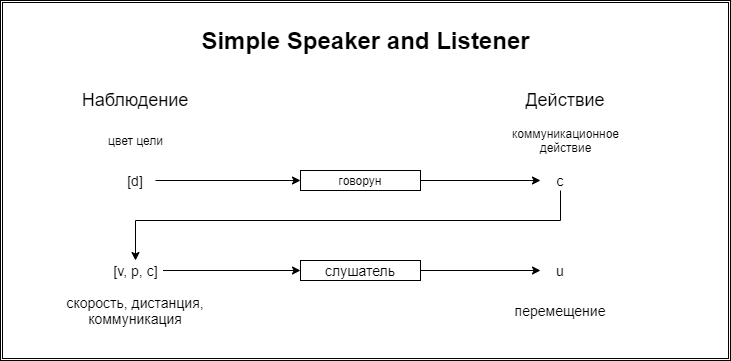
\includegraphics [scale=0.60] {my_folder/images/ch4/simple_speaker_listener.png}
    \caption{\textit{Говорун} наблюдает цвет целевого ориентира \textit{d} и издает коммуникационое действие, которое будет получено \textit{слушателем}. \textit{Слушатель} производит физическое движение.}
    \label{fig:ch4-ssl}
\end{figure}

Два агента имеют общую награду \textit{r}, которая является отрицательным евклидовым расстоянием между \textit{слушателем} и его целью. Проблема, которую необходимо решить в этом сценарии, заключается в поиске оптимальных политик для \textit{говоруна} и \textit{слушателя}, чтобы максимизировать ожидаемую награду, то есть $\max_{\pi}R(\pi)$, где

\begin{equation}
    \begin{multlined}
        R(\pi) = \mathbb{E}[\sum_{t=0}^{T}r(s_t, a_t)]
    \end{multlined}
\end{equation}

Во время обучения \textit{говорун} учится различать три ориентира и передавать целевой ориентир \textit{слушателю}. И \textit{слушатель} должен изучить закодированные высказывания, говоруна, и перейти к правильной цели.

TODO: уточнить параметры

Архитектура актор-сети \textit{говоруна} аналогична архитектуре \textit{слушателя}, каждый из которых содержит два полно связанных слоя с 64 нейронами и использует функцию активации relu. Однако их выходные слои различаются с точки зрения количества единиц и функций активации. Для \textit{говоруна} используется функция активации Gumbel-Softmax, а для слушателя - tanh. Сети критиков имеют структуру, аналогичную сетям акторов, за исключением того, что они выдают скалярное Q-значение.

\subsection{Сценарий 2}

TODO

\subsection{Сценарий 3}

TODO

\newpage
